\subsection{Gesamtarchitektur einer HTTP/Express Applikation}

\begin{frame}{Gesamtarchitektur einer HTTP/Express Applikation}{Technischer Überblick}
  \begin{center}
    \begin{figure}
    \par\bigskip
    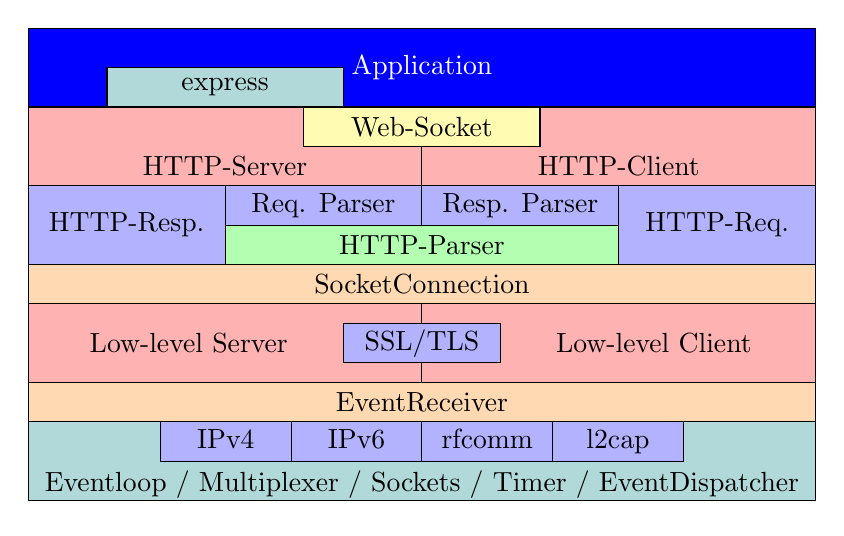
\begin{tikzpicture}
      \node[outer sep=0, draw, fill=teal!30, minimum width=10cm, minimum height=1cm] (em) {};
      \draw (em.north) node[outer sep=0, inner sep=0, anchor=north east, draw, fill=blue!30, minimum height=0.5cm, minimum width=1.66cm] (ip6) {\strut IPv6};
      \draw (em.north) node[outer sep=0, inner sep=0, anchor=north west, draw, fill=blue!30, minimum height=0.5cm, minimum width=1.66cm] (rfcomm) {\strut rfcomm};
      \draw (rfcomm.east) node[outer sep=0, inner sep=0, anchor=west, draw, fill=blue!30, minimum height=0.5cm, minimum width=1.66cm] (l2cap) {\strut l2cap};
      \draw (ip6.west) node[outer sep=0, inner sep=0, anchor=east, draw, fill=blue!30, minimum height=0.5cm, minimum width=1.66cm] (ip4) {\strut IPv4};
      \draw (em.center) node[anchor=north] {Eventloop / Multiplexer / Sockets / Timer / EventDispatcher};


      \draw (em.north) node[outer sep=0, inner sep=0, anchor=south, draw, fill=orange!30, minimum width =10cm, minimum height=0.5cm](ev) {};

      \draw (ev.north) node[anchor=north] {EventReceiver};

      \draw (ev.north west) node[outer sep=0, anchor=south west, draw, fill=red!30, minimum width=5cm, minimum height=1cm] (lls) {};
      \draw (ev.north east) node[outer sep=0, anchor=south east, draw, fill=red!30, minimum width=5cm, minimum height=1cm] (llc) {};
      \draw (lls.east) node[outer sep=0, inner sep=0, anchor=center, draw, fill=blue!30, minimum width=2cm, minimum height=0.5cm] (ssl) {SSL/TLS};
      \draw (ssl.west) node[outer sep=20, inner sep=0, anchor=east] (llst) {Low-level Server};
      \draw (ssl.east) node[outer sep=20, inner sep=0, anchor=west] (llct) {Low-level Client};
      \draw (lls.north east) node[anchor=south, draw, fill=orange!30, inner sep=0, outer sep=0, minimum width=10cm, minimum height=0.5cm] (sc) {SocketConnection};
      \draw (sc.north) node [anchor=south, outer sep=0, inner sep=0, draw, fill=green!30, minimum width=5cm, minimum height=0.5cm] (http-p) {HTTP-Parser};
      \draw (http-p.south west) node[anchor=south east, outer sep=0, inner sep=0, draw, fill=blue!30, minimum width=2.5cm, minimum height=1cm] (http-res) {HTTP-Resp.};
      \draw (http-p.south east) node[anchor=south west, outer sep=0, inner sep=0, draw, fill=blue!30, minimum width=2.5cm, minimum height=1cm] (http-res) {HTTP-Req.};
      \draw (http-p.north west) node[anchor=south west, outer sep=0, inner sep=0, draw, fill=blue!30, minimum width=2.5cm, minimum height=0.5cm] (http-reqp) {Req. Parser};
      \draw (http-p.north east) node[anchor=south east, outer sep=0, inner sep=0, draw, fill=blue!30, minimum width=2.5cm, minimum height=0.5cm] (http-respp) {Resp. Parser};
      \draw (http-respp.north west) node[outer sep=0, inner sep=0, anchor=south west, fill=red!30, draw, minimum width=5cm, minimum height=1cm] (http-c) {};
      \draw (http-respp.north west) node[outer sep=0, inner sep=0, anchor=south west, minimum width=5cm, minimum height=0.5cm]  {HTTP-Client};
      \draw (http-reqp.north east) node[outer sep=0, inner sep=0, anchor=south east, fill=red!30, draw, minimum width=5cm, minimum height=1cm] (http-s) {};
      \draw (http-reqp.north east) node[outer sep=0, inner sep=0, anchor=south east, minimum width=5cm, minimum height=0.5cm]  {HTTP-Server};
      \draw (http-s.north east) node[anchor=north, outer sep=0, inner sep=0, minimum width=3cm, minimum height=0.5cm, draw, fill=yellow!30] (ws) {Web-Socket};
      \visible<2>{\draw (ws.north) node[anchor=south, outer sep=0, inner sep=0, draw, fill=blue, minimum width=10cm, minimum height=1cm] {\color{white}Application};}
      \draw (http-s.north) node[anchor=south, draw, fill=teal!30, outer sep=0, inner sep=0, minimum height=0.5cm, minimum width=3cm] {express};
    \end{tikzpicture}
    \caption{Gesamtarchitektur}
  \end{figure}
  \end{center}
\end{frame}
